\def\SECTION{1.5 Angles}
\documentclass[aspectratio=169,14pt]{beamer}
\usepackage[T1]{fontenc}
\usepackage{mathpazo}
\usepackage{amsmath,amssymb}
\usepackage{tikz}
\usetikzlibrary{arrows.meta,calc,decorations.pathreplacing}
\definecolor{fblue}{HTML}{1F4E79}
\definecolor{fteal}{HTML}{0F7C7C}
\definecolor{fgold}{HTML}{C9962B}
\definecolor{fred}{HTML}{B3261E}
\definecolor{fink}{HTML}{16233B}
\definecolor{fsoft}{HTML}{EEF3F8}
\definecolor{fgoldsoft}{HTML}{FBF1DC}
\setbeamertemplate{navigation symbols}{}
\setbeamercolor{normal text}{fg=fink}
\setbeamercolor{frametitle}{fg=fblue}
\setbeamerfont{frametitle}{series=\bfseries,size=\Large}
\setbeamercolor{structure}{fg=fteal}
\setbeamertemplate{itemize item}{\color{fteal}$\blacktriangleright$}
\setbeamertemplate{frametitle}{\vspace{6pt}\insertframetitle\par\vspace{-2pt}{\color{fgold}\rule{2.2cm}{2pt}}}
\setbeamertemplate{footline}{\hspace{0.6cm}{\color{fblue}\scriptsize\bfseries Fang\textcolor{fteal}{Math}}\hfill{\scriptsize\color{gray}\SECTION\quad\insertframenumber}\hspace{0.6cm}\vspace{6pt}}
\newcommand{\key}[1]{{\color{fteal}\textbf{#1}}}
\newcommand{\ans}[1]{\colorbox{fgoldsoft}{\color{fink}\ensuremath{#1}}}
\newcommand{\warn}[1]{\begin{beamercolorbox}[sep=8pt,rounded=true]{warnbox}{\color{fred}\textbf{Watch out!}}\enskip #1\end{beamercolorbox}}
\setbeamercolor{warnbox}{bg=fred!8,fg=fink}
\setbeamercolor{turnbox}{bg=fgoldsoft,fg=fink}
\setbeamercolor{defbox}{bg=fsoft,fg=fink}
\newcommand{\defn}[1]{\begin{beamercolorbox}[sep=8pt,rounded=true]{defbox}#1\end{beamercolorbox}}
\newenvironment{yourturn}{\begin{beamercolorbox}[sep=10pt,rounded=true]{turnbox}{\color{fgold}\Large\bfseries Your turn!}\quad{\small Pause the video and try it.}\par\medskip}{\end{beamercolorbox}}
\newcommand{\titleframe}[3]{%
\begin{frame}[plain]
\begin{tikzpicture}[remember picture,overlay]
\fill[fblue] (current page.north west) rectangle ([yshift=-0.9cm]current page.north east);
\node[anchor=west,text=white,font=\bfseries] at ([xshift=0.6cm,yshift=-0.45cm]current page.north west) {Fang\textcolor{fgold}{Math}};
\node[anchor=east,text=white,font=\small] at ([xshift=-0.6cm,yshift=-0.45cm]current page.north east) {Geometry $\cdot$ Chapter 1};
\end{tikzpicture}
\vfill
{\color{fteal}\large\bfseries #1}\par\medskip
{\color{fblue}\fontsize{30}{34}\selectfont\bfseries #2}\par\medskip
{\color{fgold}\rule{3cm}{3pt}}\par\bigskip
{\large #3}
\vfill
{\small\color{gray} fangmath.com $\cdot$ YouTube @3SMath}
\end{frame}}
\newcommand{\closeframe}[1]{%
\begin{frame}{Remember}
#1
\vfill
\begin{center}{\color{fblue}\large\bfseries Now practice at your level:}\par\smallskip
{\Large\color{fteal}\bfseries fangmath.com} \enskip{\color{gray}$\to$ Geometry $\to$ Chapter 1}\end{center}
\end{frame}}

\usepackage{pgfplots}\pgfplotsset{compat=1.17}
\newcommand{\grid}[4]{\draw[step=1,gray!25] (#1,#2) grid (#3,#4);\draw[-{Stealth},gray] (#1,0)--(#3+0.3,0) node[right]{\small$x$};\draw[-{Stealth},gray] (0,#2)--(0,#4+0.3) node[above]{\small$y$};}
\usetikzlibrary{angles,quotes}
\begin{document}
\titleframe{Lesson 1.5}{Angles}{Measure, classify, add --- and the angle pairs}

\begin{frame}{Four kinds of angles}
\begin{columns}[b]
\begin{column}{0.24\textwidth}\centering
\tikz[baseline=0]{\draw[very thick,-{Stealth}] (0,0)--(1.6,0); \draw[very thick,-{Stealth}] (0,0)--(55:1.6); \draw[fteal,thick] (0.45,0) arc (0:55:0.45);}\par\medskip{\color{fblue}\bfseries Acute}\par\small less than $90^\circ$
\end{column}
\begin{column}{0.24\textwidth}\centering
\onslide<2->{\tikz[baseline=0]{\draw[very thick,-{Stealth}] (0,0)--(1.6,0); \draw[very thick,-{Stealth}] (0,0)--(0,1.6); \draw[fteal,thick] (0.35,0)--(0.35,0.35)--(0,0.35);}\par\medskip{\color{fblue}\bfseries Right}\par\small exactly $90^\circ$}
\end{column}
\begin{column}{0.24\textwidth}\centering
\onslide<3->{\tikz[baseline=0]{\draw[very thick,-{Stealth}] (0,0)--(1.6,0); \draw[very thick,-{Stealth}] (0,0)--(130:1.6); \draw[fteal,thick] (0.45,0) arc (0:130:0.45);}\par\medskip{\color{fblue}\bfseries Obtuse}\par\small between $90^\circ$ and $180^\circ$}
\end{column}
\begin{column}{0.24\textwidth}\centering
\onslide<4->{\tikz[baseline=0]{\draw[very thick,{Stealth}-{Stealth}] (-1.2,0)--(1.2,0); \fill (0,0) circle(2pt); \draw[fteal,thick] (0.4,0) arc (0:180:0.4);}\par\medskip{\color{fblue}\bfseries Straight}\par\small exactly $180^\circ$}
\end{column}
\end{columns}
\end{frame}

\begin{frame}{Reading an angle's name}
\begin{columns}[c]
\begin{column}{0.45\textwidth}\centering
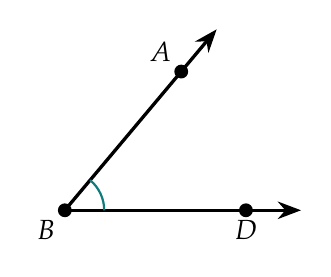
\begin{tikzpicture}[scale=1]
\draw[very thick,-{Stealth}] (0,0)--(3,0); \draw[very thick,-{Stealth}] (0,0)--(50:3);
\fill (0,0) circle(2.5pt) node[below left]{$B$} (2.3,0) circle(2.5pt) node[below]{$D$} (50:2.3) circle(2.5pt) node[above left]{$A$};
\draw[fteal,thick] (0.5,0) arc (0:50:0.5);
\end{tikzpicture}
\end{column}
\begin{column}{0.53\textwidth}
{\Large $\angle ABD$}\par\medskip
The \key{vertex} is the \key{middle} letter: $B$.\par\medskip
{\small\color{gray} $\angle ABD$ and $\angle DBA$ name the same angle.}
\end{column}
\end{columns}
\end{frame}

\begin{frame}{Angle Addition Postulate}
\begin{columns}[c]
\begin{column}{0.45\textwidth}\centering
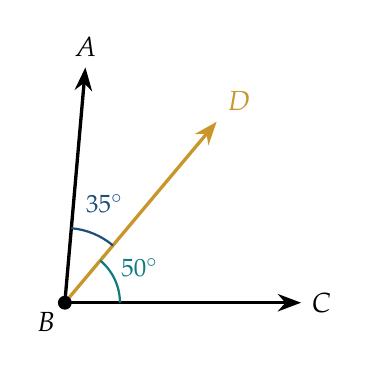
\begin{tikzpicture}[scale=1]
\draw[very thick,-{Stealth}] (0,0)--(3,0) node[right]{$C$}; \draw[very thick,-{Stealth}] (0,0)--(85:3) node[above]{$A$};
\draw[very thick,-{Stealth},fgold] (0,0)--(50:3) node[above right]{$D$};
\fill (0,0) circle(2.5pt) node[below left]{$B$};
\onslide<2->{\draw[fteal,thick] (0.7,0) arc (0:50:0.7); \node[fteal] at (25:1.05){\small $50^\circ$}; \draw[fblue,thick] (50:0.95) arc (50:85:0.95); \node[fblue] at (68:1.35){\small $35^\circ$};}
\end{tikzpicture}
\end{column}
\begin{column}{0.53\textwidth}
$D$ is inside $\angle ABC$.\par\medskip
\onslide<2->{$m\angle ABD = 35^\circ,\ m\angle DBC = 50^\circ$}\par\medskip
\onslide<3->{$m\angle ABC = 35 + 50 = \ans{85^\circ}$\par{\small\color{gray} the two small angles fill the big one}}\par\medskip
\onslide<4->{$85^\circ < 90^\circ$: \ \key{acute}}
\end{column}
\end{columns}
\end{frame}

\begin{frame}{With algebra}
$D$ is inside $\angle ABC$.\quad $m\angle ABD = 2x + 5,\quad m\angle DBC = 3x,\quad m\angle ABC = 80^\circ.$\par\medskip
Find $m\angle DBC$.\par\bigskip
\onslide<2->{$(2x + 5) + 3x = 80$ \qquad{\small\color{gray} part $+$ part $=$ whole}}\par\smallskip
\onslide<3->{$5x + 5 = 80 \;\Rightarrow\; 5x = 75 \;\Rightarrow\; x = 15$}\par\smallskip
\onslide<4->{$m\angle DBC = 3(15) = \ans{45^\circ}$ \qquad{\small\color{gray} check: $35 + 45 = 80$ \checkmark}}
\end{frame}

\begin{frame}{Angle pairs}
\begin{columns}[c]
\begin{column}{0.48\textwidth}\centering
\onslide<1->{\tikz{\draw[very thick] (0,0)--(2,0); \draw[very thick] (0,0)--(0,2); \draw[very thick,fteal] (0,0)--(35:2); \node at (17:0.9){\small$35^\circ$}; \node at (62:0.9){\small$55^\circ$};}\par\medskip
\key{Complementary}: add to $90^\circ$}
\end{column}
\begin{column}{0.48\textwidth}\centering
\onslide<2->{\tikz{\draw[very thick] (-2,0)--(2,0); \draw[very thick,fgold] (0,0)--(65:2); \node at (32:0.8){\small$65^\circ$}; \node at (122:0.8){\small$115^\circ$};}\par\medskip
\key{Supplementary}: add to $180^\circ$}
\end{column}
\end{columns}
\bigskip
\onslide<3->{\defn{\centering \textbf{C} comes before \textbf{S} in the alphabet --- just like $90$ comes before $180$.}}
\end{frame}

\begin{frame}{Find the missing angle}
\onslide<1->{Supplement of $65^\circ$?}\par\smallskip
\onslide<2->{$180 - 65 = \ans{115^\circ}$}\par\bigskip
\onslide<3->{Complement of $65^\circ$? \par\smallskip $90 - 65 = \ans{25^\circ}$}
\end{frame}

\begin{frame}{Vertical angles and linear pairs}
\begin{columns}[c]
\begin{column}{0.45\textwidth}\centering
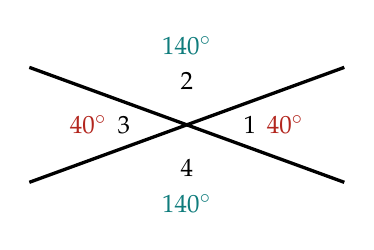
\begin{tikzpicture}[scale=1]
\draw[very thick] (-2,-0.73)--(2,0.73); \draw[very thick] (-2,0.73)--(2,-0.73);
\node at (0.8,0){\small$1$}; \node at (-0.8,0){\small$3$}; \node at (0,0.55){\small$2$}; \node at (0,-0.55){\small$4$};
\onslide<3->{\node[fred] at (1.25,0){\small$40^\circ$}; \node[fred] at (-1.25,0){\small$40^\circ$}; \node[fteal] at (0,1){\small$140^\circ$}; \node[fteal] at (0,-1){\small$140^\circ$};}
\end{tikzpicture}
\end{column}
\begin{column}{0.53\textwidth}
\onslide<1->{\key{Vertical angles} are across from each other, and they are \textbf{equal}: $\angle 1 = \angle 3$.}\par\medskip
\onslide<2->{\key{Linear pair}: side by side on a line, they add to $180^\circ$: $\angle 1 + \angle 2 = 180^\circ$.}\par\medskip
\onslide<3->{If $\angle 1 = 40^\circ$: \ $\angle 3 = 40^\circ$, \ $\angle 2 = \angle 4 = 140^\circ$.}
\end{column}
\end{columns}
\end{frame}

\begin{frame}{}
\begin{yourturn}
$\angle 1$ and $\angle 2$ are supplementary. \quad $m\angle 1 = 4x + 20,\quad m\angle 2 = 2x + 40$.\par\smallskip
Find $x$ and both angles.
\end{yourturn}
\pause\bigskip
$(4x + 20) + (2x + 40) = 180 \;\Rightarrow\; 6x + 60 = 180 \;\Rightarrow\; x = \ans{20}$\par\medskip
$m\angle 1 = \ans{100^\circ}$, \quad $m\angle 2 = \ans{80^\circ}$ \qquad{\small\color{gray} $100 + 80 = 180$ \checkmark}
\end{frame}

\closeframe{\begin{itemize}\setlength\itemsep{8pt}
\item Acute $< 90^\circ$, right $= 90^\circ$, obtuse between, straight $= 180^\circ$.
\item The vertex is the \key{middle} letter. Small angles add up to the big one.
\item \key{Complementary} $90^\circ$, \key{supplementary} $180^\circ$, \key{vertical} angles are equal.
\end{itemize}}
\end{document}
